\documentclass[tikz,border=6pt]{standalone}
\usepackage{ctex}
\usepackage{graphicx}
\usepackage{subcaption}
\usepackage{tikz}
\begin{document}
\begin{minipage}{0.98\textwidth}
\centering
\begin{subfigure}[t]{0.48\textwidth}
  \centering
  
\includegraphics[width=\textwidth]{real-training-images/training_curves.png}
  \caption{CAN-CNN(64x9) 训练/验证曲线（真实训练产物）}
\end{subfigure}
\hfill
\begin{subfigure}[t]{0.48\textwidth}
  \centering
  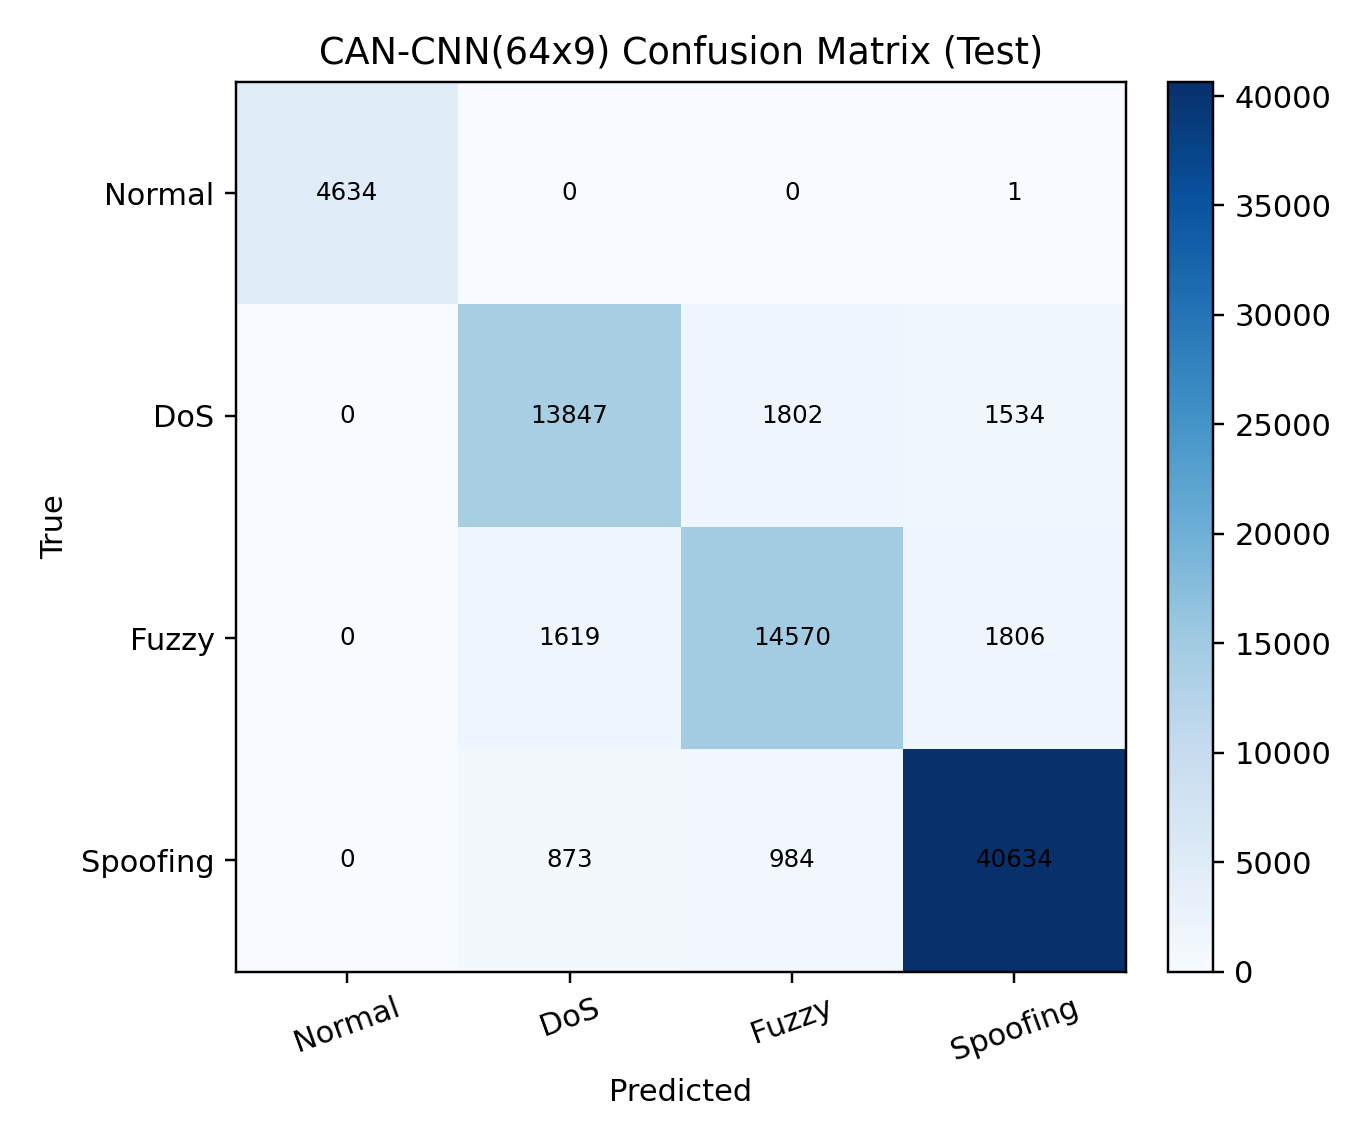
\includegraphics[width=\textwidth]{real-training-images/confusion_matrix_can_cnn64.png}
  \caption{测试集混淆矩阵（由 \texttt{eval\_metrics.json} 生成）}
\end{subfigure}

\vspace{0.8em}

\begin{subfigure}[t]{0.60\textwidth}
  \centering
  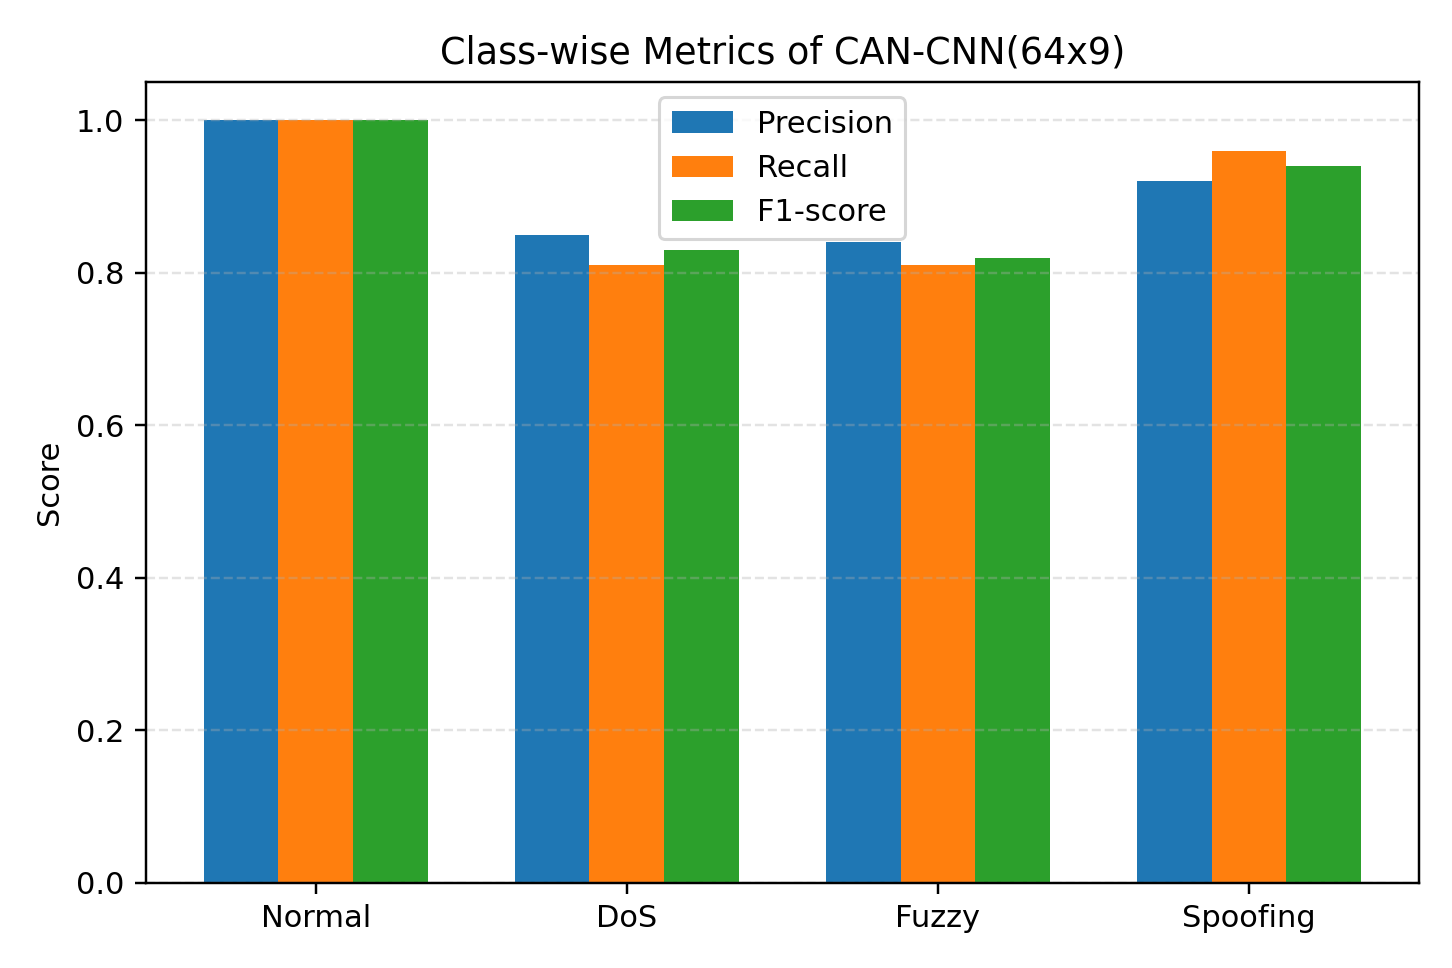
\includegraphics[width=\textwidth]{real-training-images/class_metrics_can_cnn64.png}
  \caption{各类别 Precision/Recall/F1（由评估结果生成）}
\end{subfigure}

\vspace{0.8em}

\begin{subfigure}[t]{0.88\textwidth}
  \centering
  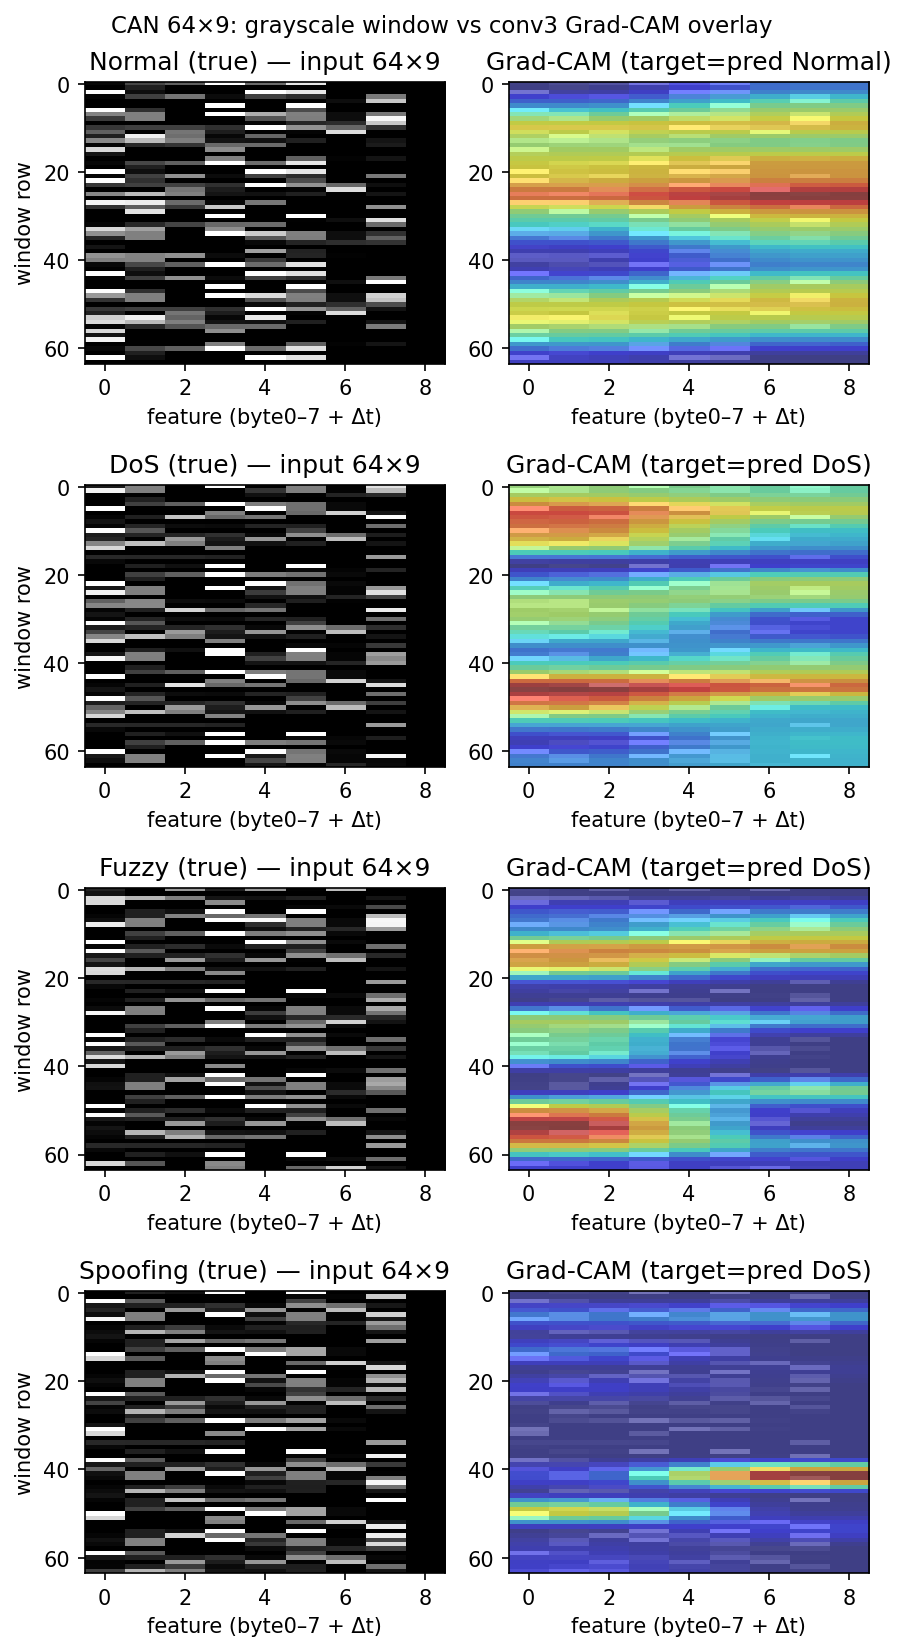
\includegraphics[width=\textwidth]{real-training-images/analysis_result.png}
  \caption{Grad-CAM 可解释性结果：左列为 64x9 输入灰度图，右列为针对预测类别的 \texttt{conv3} 热力响应}
\end{subfigure}

\vspace{0.4em}

\begin{tikzpicture}
  \node[draw=black!35, rounded corners=2mm, fill=blue!6, align=left, inner sep=5pt] {
  该图组仅基于 \texttt{can\_cnn\_64x9} 训练、测试与 Grad-CAM 解释结果，不包含二维/跨域链路模型图。};
\end{tikzpicture}
\end{minipage}
\end{document}
